\section{Discussions}

\label{sec:disc}


\subsection{Analysis on the architecture}

Assume that we have a network with $L$ layers, and skip connections are passed every
layer in the first half of the network. For the convenience of presentation, we
denote $F_c$ and $F_d$  the convolution and deconvolution operation in each layer
and do not use ReLU. According to the architecture described in the last section,
we can obtain the output of the $i$-th layer as follows:
\begin{equation}
   X_i = \left\{
   \begin{array}{ll}
   X_{L-i} + F_d(X_{i-1}), & i\geq L/2;\\
   F_c(X_{i-1}).           & i<L/2.
   \end{array} \right.
\label{eq5}
\end{equation}
It is easy to observe that our skip connections indicate identity mapping.
The output of the network is:
\begin{equation}
X_L = X_0 + F_d(X_{L-1}).
\end{equation}
Recursively, we can compute $X_L$ more specifically as follows according to Equation \eqref{eq5}:
\begin{equation}
\begin{aligned}
X_L & = X_0 + F_d(X_{L-1}) \\
    & = X_0 + F_d(X_1 + F_d(X_{L-2})) \\
    & = X_0 + F_d(X_1) + F_d^2(X_2+F_d(X_{L-3})) \\
    & ......   \\
    & = X_0 + F_d(X_1) + F_d^2(X_2) + ... +F_d^{L/2-1}(X_{L/2-1}) \\
    & + F_d^{L/2}(X_{L/2}).
\end{aligned}
\label{eq6}
\end{equation}
Since $F_d^{L/2}(X_{L/2})$ can be expressed as $F_d^{L/2}(F_c^{L/2}(X_0))$, we convert Equation \eqref{eq6} as:
\begin{equation}
X_L = F_d^{L/2}(F_c^{L/2}(X_0)) + \sum_{i=0}^{L/2-1} F_d^i(X_i).
\label{eq7}
\end{equation}
In Equation \eqref{eq7}, the term $F_d^{L/2}(F_c^{L/2}(X_0))$ is actually the output
of the given network without skip connections. The difference here is that by adopting
the skip connection, we decode each feature maps $X_i, 0\leq i <L/2$ in the first half
network and integrate them to the output. The most significant benefit is that they carry
important image details, which helps to reconstruct clean image. Moreover, the term
$\sum_{i=0}^{L/2-1} F_d^i(X_i)$ indicates that these details are represented at
different levels. It is intuitive  to see the following fact. It may not be easy to tell what information
 is needed for
reconstructing clean images using only one feature maps encoding the image abstraction;
but much easier if there are multiple feature maps encoding different levels of image abstraction.



\subsection{Gradient back-propagation}

For back-propagation, a layer receives gradients from the layers that it is connected to.
As an example shown in Figure \ref{fig4}, $X$ is the input of the first layer,
after two convolutional layers $c1$ and $c2$, the output is $X_1$. To update the parameters
represented as $\theta_2$ of $c2$, we compute the derivative of $\mathcal{L}$ with
respect to $\theta_2$ as follows:
\begin{equation}
\nabla_{\theta_2}\mathcal{L}(\theta_2) = \frac{\partial\mathcal{L}}{\partial X_1}\frac{\partial X_1}{\partial\theta_2} + \frac{\partial\mathcal{L}}{\partial X_2}\frac{\partial X_2}{\partial\theta_2}
\label{eq2}
\end{equation}
where using $X_1$ and $X_2$ is only for the clarity of presentation, they are essentially
the same. We can further formulate \eqref{eq2} as:
\begin{equation}
\nabla_{\theta_2}\mathcal{L}(\theta_2) = \frac{\partial\mathcal{L}}{\partial X_4}\frac{\partial X_4}{\partial X_3}\frac{\partial X_3}{\partial X_1}\frac{\partial X_1}{\partial\theta_2} + \frac{\partial\mathcal{L}}{\partial X_4}\frac{\partial X_4}{\partial X_2}\frac{\partial X_2}{\partial\theta_2}.
\label{eq3}
\end{equation}
Only $\frac{\partial\mathcal{L}}{\partial X_4}\frac{\partial X_4}{\partial X_3}\frac{\partial X_3}{\partial X_1}\frac{\partial X_1}{\partial\theta_2}$ is computed if we do not use skip connections, and its magnitide
 may become very
small after back-propagating through many layers from the top in very deep networks.
However, $\frac{\partial\mathcal{L}}{\partial X_4}\frac{\partial X_4}{\partial X_2}\frac{\partial X_2}{\partial\theta_2}$
carries larger gradients since it does not have to go through layers of $d2$, $d1$, $c4$ and $c3$ in this example.
Thus with the first term only, it is more unlikely to approach zero grdients.
 As we can see, the skip connection helps to update
the filters in bottoms layers, and thus makes training easier.

\subsection{Training with symmetric skip connections}

The aim of restoration is to eliminate corruption while preserving the image details
as mush as possible. Previous works typically use shallow networks for low-level image
restoration tasks. The reason may be that deeper networks can destroy the image details,
which is undesired for pixel-wise dense regression. Even worse, using very deep networks
may easily suffer from training issues such as gradient vanishing. Using skip
connections in a very deep network can address both  of the above two problems.

Firstly, we design experiments to show that using skip connections is beneficial for
image detail presering. Specifically, two networks are trained for image denoising
with a noise level of $\sigma=70$.

(a) In the first network, we use 5 layers of $3\times3$ convolution with stride 3.
The input size of training data is $243\times243$, which results in a vector after
5 layers of convolution, encoding the very high level abstraction of the image. Then
deconvolution is used to recover the input from the feature vector. The results are
shown in Figure \ref{fig5}. We can observe that it is challenging for deconvolution to recover
details from only a vector encoding the abstraction of the input. This phenomenon
implies that  simply using deep networks for image restoration may not lead to satisfactory results.
%
%

(b) The second network uses the same settings as the first one, but adding
skip connections. The results are show in Figure \ref{fig5}. Compared to the first
network, the one with skip connections can recover the input and achieves much
better PSNR values. This is easy to understand since the feature maps with abundant
details at bottom layers are directly passed to the top layers.

\begin{figure}[htb!]
\centering
\includegraphics[width=0.48\textwidth]{recover-detail-psnr}
\caption{Recovering image details using deconvolution and skip connections. Skip
connections are beneficial in recovering image details.}
\label{fig5}
\end{figure}

Secondly, we train and compare five different networks to show that using skip
connections help to back-propagate gradient in training to better fit the end-to-end
mapping, as shown in Figure \ref{fig6}. The five networks are: 10, 20 and 30 layer
networks without skip connections;  and 20, 30 layer networks with skip connections.
As  can be seen, the training loss increases when the network going deeper without
shortcuts (similar phenomenon is also observed in \cite{DBLP:journals/corr/HeZRS15}).
On the validation set, deeper networks without shortcuts achieve lower PSNR and we
even observe over-fitting for the 30-layer network. These results may be due to  the
gradient vanishing problem. However, we obtain smaller training errors on the training set and
higher PSNR and better generalization capability on the testing set when using skip connections.


\begin{figure}[b!]
\centering
\includegraphics[width=0.48\textwidth]{10-20-20R-30-30R-loss}
\caption{The training loss on the training set during training.}
\label{fig6}
\end{figure}



\subsection{Comparison with the deep residual network \cite{DBLP:journals/corr/HeZRS15}}

One may use different types of skip connections in our network. A straightforward
alternate is that in ~\cite{DBLP:journals/corr/HeZRS15}. In ~\cite{DBLP:journals/corr/HeZRS15},
 skip connections are added to divide the network into sequential blocks. A benefit
of our model is that our skip connections have element-wise correspondence, which can be
very important in pixel-wise prediction problems such image denoising. We carry out
experiments to compare these two types of skip connections. Here the block size indicates
the span of the connections. The results are shown in Figure \ref{fig8}. We can observe
that our connections often converge to a better optimum, demonstrating that element-wise
correspondence can be important. Meanwhile, our long range skip connections pass the image
detail directly from bottom layers to top layers. If we use the skip connection type in
~\cite{DBLP:journals/corr/HeZRS15}, the network may still lose some image details.


\begin{figure}[t!]
\centering
\includegraphics[width=0.48\textwidth]{connection-type-psnr}
\caption{Comparisons of skip connections in ~\cite{DBLP:journals/corr/HeZRS15} and our
model, where ``Block-$i$-RED" is the connections in our model with block size $i$ and
``Block-$i$-He et al." is the connections in He et al.~\cite{DBLP:journals/corr/HeZRS15}
with block size $i$; The PSNR values on the validation set during training: the PSNR at
the last iteration for the curves are: 25.08, 24.59, 25.30 and 25.21.}
\label{fig8}
\end{figure}


\subsection{Testing efficiency}

To apply deep learning models on devices with limited computing power such as mobile
phones, one has to speed-up the testing phase. For our network, we propose to use
down-sampling in convolutional layers to reduce the size of the feature maps. In order
to obtain an output of the same size as the input, deconvolution is used to up-sample
the feature maps in the symmetric deconvolutional layers.  Thus, the testing
efficiency can be well improved with almost negligible  performance degradation.


In specific, we use stride $=$ 2 in convolutional layers to down-sample the feature maps.
Down-sampling at different convolutional layers are tested on image denoising, as shown
in Figure \ref{fig16}. We test an image of size 160$\times$240 on an i7-2600 CPU, the testing
time for ``no down-sample", ``down-sample at conv1", ``down-sample at conv5",
``down-sample at conv9", "down-sample at conv5,9" are 3.17s, 0.84s, 1.43s, 2.00s and
1.17s respectively.

The main observation is that the testing PSNRs may slightly degrade according to the scale
reduction of the feature map in the entire network. The down-sampling in the first
convolutional layer reduces the size of the feature maps to 1/4, which leads to alomst 4x
faster in testing, but the PSNR only degrades less than 0.1 compared to the network without
down-sampling. The down-sampling in "conv9" reduces 1/3 of the testing time, but the
performance is almost as well as that without down-sampling. As a result, an "earlier"
down-sampling may lead to slightly worse performance, but it achieves much faster testing
efficiency. It should be a trade-off in different application situations.


\begin{figure}[t!]
\centering
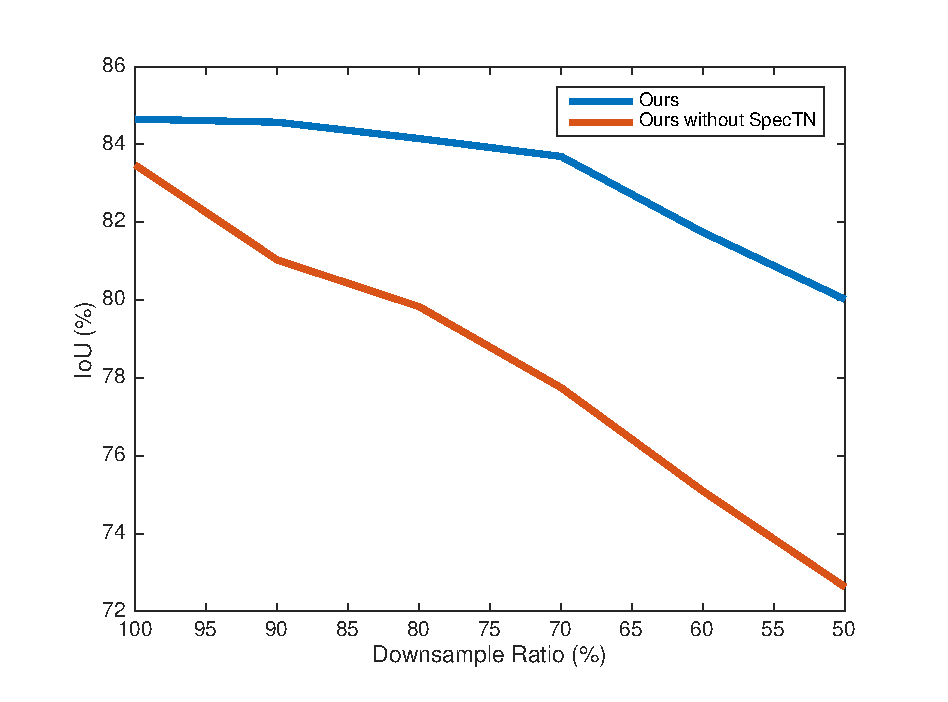
\includegraphics[width=0.48\textwidth]{downsample}
\caption{The PSNRs on the validation set with different down-sampling strategies.
``down-sample at conv-i" denotes that down-sampling is used in the $i$th convolutional
layer, and up-sampling is used in its symmetric deconvolutional layer.}
\label{fig16}
\end{figure}

